

% Order of presentation:  Figure 1 (best times), Figure 6 (worst times),  Figure 12 (com todas as entradas), Figure 13 (real). 
% Ricardo Rocha, June 30, 2013

%\documentclass[times,10pt,twocolumn]{article} 
%\usepackage{latex8}
%\usepackage{times}

%\documentclass[10pt]{IEEEtran}
\documentclass[conference]{IEEEtran}
% allow \thanks
\IEEEoverridecommandlockouts

\usepackage[pdftex]{graphicx}
%%\usepackage{epsf}
\usepackage[tight,footnotesize]{subfigure}
%%\usepackage{multirow}
%%\usepackage{tabularx}
%\usepackage{setspace}
\usepackage[ruled,linesnumbered]{algorithm2e}
%%\usepackage{algorithm2e}
\usepackage{amsmath}
%\usepackage{fullpage}
\input{rr-common.tex}

%\pagestyle{empty}
\pagestyle{plain}


% Colors on or off: Pick ONE
\renewcommand{\ifColorText}[2]{\textcolor{#1}{#2}}  % Colors ON
%\renewcommand{\ifColorText}[2]{{#2}}                % Colors OFF

% Comments on or off: Pick ONE
%\renewcommand{\ifComments}[1]{{#1}}                 % Comments ON
%\renewcommand{\ifComments}[1]{\REM{#1}}             % Comments OFF

\newif\ifComments
\Commentstrue

\ifComments
\newcommand{\chek}[1]{\noindent\textcolor{red}{Check: {#1}}}
\newcommand{\jna}[1]{\noindent\textcolor{blue}{Nelson: {#1}}}
\newcommand{\rlar}[1]{\noindent\textcolor{green}{Ricardo: {#1}}}
\newcommand{\paul}[1]{\noindent\textcolor{magenta}{Berube: {#1}}}
\newcommand{\bruno}[1]{\noindent\textcolor{magenta}{Bruno: {#1}}}
\newcommand{\rem}[1]{\noindent\textcolor{red}{\st{#1}}}
\newcommand{\new}[1]{\noindent\textcolor{blue}{ {#1}}}
\newcommand{\ed}[1]{\noindent\textcolor{red}{ {#1}}}
\newcommand{\short}[1]{\noindent\textcolor{blue}{ {#1}}}
\else
\newcommand{\chek}[1]{}
\newcommand{\jna}[1]{}
\newcommand{\rlar}[1]{}
\newcommand{\paul}[1]{}
\newcommand{\bruno}[1]{}
\newcommand{\rem}[1]{}
\newcommand{\new}[1]{#1}
\newcommand{\new}[1]{\noindent\textcolor{blue}{ {#1}}}
\newcommand{\ed}[1]{#1}
\newcommand{\short}[1]{}
\fi

\newcommand{\abbrev}[2][Blue]{\ifColorText{#1}{\ensuremath{\mathrm{#2}}}}

\def\llvm{{\ifColorText{Red}{{\tt LLVM}}}}
\def\Never{{\ifColorText{Red}{{\tt Never}}}}
\def\PP{{\ifColorText{Orange}{PP}}}
\def\CP{{\ifColorText{RoyalBlue}{CP}}}
\def\CEP{{\ifColorText{RoyalBlue}{CEP}}}
\def\CPP{{\ifColorText{RoyalBlue}{CPP}}}
\def\HN{{\ifColorText{OliveGreen}{HN}}}
\def\CG{{\ifColorText{Periwinkle}{CG}}}
\def\CFG{{\ifColorText{Fuchsia}{CFG}}}
\def\FDO{{\ifColorText{Magenta}{FDO}}}
\def\DF{{\ifColorText{Blue}{\ensuremath{\mathrm{DF}}}}}
\def\FDI{{\ifColorText{Magenta}{FDI}}}
\def\CS{\abbrev{CS}}

\newcommand{\DFact}[2]{{\ifColorText{Blue}{\ensuremath{\mathrm{\DF}_{{#1}\rightarrow {#2}}}}}}

\newcommand{\blt}[1]{\ensuremath{t_\emptyset}(#1)}

\begin{document}
\thispagestyle{empty}

\title{A Methodology for the Evaluation of Code Transformations Based on Feedback-Directed Optimizations}

%\pagenumbering{arabic}

%\authorinfo{\ }{\ }{\ }
\author{\IEEEauthorblockN{Ricardo Luis de Azevedo da Rocha\thanks{This research was done while the nth author was in a sabbatical year at the University of Alberta, supported by grant 2011/17096-5 from the Funda\c{c}\~{a}o de Amparo \`{a} Pesquisa do Estado de S\~{a}o Paulo -- FAPESP.}}
\IEEEauthorblockA{Dept. of Computing Engineering\\
University of Sao Paulo and \\ Dept. of Computing Science \\ University of Alberta\\
Edmonton, Alberta, T6G 2E8, Canada\\
Email: rlarocha@usp.br\\ \hspace{53pt}azevedod@ualberta.ca}
\and
\IEEEauthorblockN{Paul Berube}
\IEEEauthorblockA{Dept. of Computing Science\\
University of Alberta\\
Edmonton, Alberta, T6G 2E8, Canada\\
Email: pberube@ualberta.ca}
\and
\IEEEauthorblockN{Bruno Rosa}
\IEEEauthorblockA{Dept. of Computing Science\\
University of Alberta\\
Edmonton, Alberta, T6G 2E8, Canada\\
Email: brosa@ualberta.ca}
\and
\IEEEauthorblockN{Jos\'{e} Nelson Amaral\thanks{This research is supported by fellowships and grants from the Natural Sciences and Engineering Research Council of Canada (NSERC), the Informatics Circle of Research Excellence (iCORE), and the Canadian Foundation for innovation (CFI).}}
\IEEEauthorblockA{Dept. of Computing Science\\
University of Alberta\\
Edmonton, Alberta, T6G 2E8, Canada\\
Email: amaral@cs.ualberta.ca}}


\maketitle

\begin{abstract}

The usual way to do research in compilers, moreover in Feedback Directed Optimization is to construct a framework and devise an experiment based on single-run input training and single data testing. Recently some researchers have argued about the reliability of such experiments, and developed other approaches to this problem. Usually using repetition of experiments and collecting data to perform a reliable statistical analysis. This paper also discusses these issues and aims to construct an experiment to show a false speedup from actual data. This was done by just ignoring the multiple run strategy and literally selecting parts of the collected data to show that, in a single-run scheme, it can happen. As conclusion the paper states that the only way to avoid these problems is to define and use a reliable methodology based on solid statistical measurements. In this paper the methodology called {\em combined profiling} (\CP) is also presented, and it is shown that employing it can generate more reliable results. \FDI\ decisions are shown to be more accurate using \CP\ instead of single-run evaluation.

\end{abstract}

\section{Introduction}
	\label{sec:intro}
	
Research in compiler transformations often demonstrates heroic efforts in both the identification and abstract analysis of opportunities to improve program efficiency, and in the concrete implementation of these ideas.  However, standard practices at the evaluation stage of the scientific process are modest at best, perhaps because code transformations have a long history of providing significant benefits in practical, every-day situations.  In most cases, compilers are evaluated using a collection of programs, with each program evaluated using a timing run on a single evaluation input.  The deficiencies of this evaluation process are particularly prevalent, and especially disconcerting, when {\it feedback-directed optimization} (\FDI) is used to guide a transformation.  In this scenario, instrumentation is inserted into the program during an initial compilation in order to collect a profile of the run-time behavior of the program during one or more training runs.  The profile is used in a second compilation of the program to help the compiler assess the benefit of code transformation opportunities.  The current standard practice for evaluating an \FDI\ compiler uses the profile of a single-training input to guide transformations, and evaluates the transformed program with a single evaluation input.  These standard practices set program inputs as controlled variables.  However, performance evaluation should be generalizable to real-world program workloads. Consequently, the program-input dimensions of a rigorous evaluation of compiler performance must be manipulated variables.

%===================== FDI and inlining

Previous work has not addressed the problem of representing and utilizing multi-run profiles.  An \FDI\ compiler should not simply add or average profiles from multiple runs, because such a profile does not provide any information about the variations in program behaviors observed between different inputs. ~\cite{BerubePhD} uses {\it Combined Profiling} (\CP) to merge the profiles from multiple runs into a distribution model that allows code transformations to consider cross-run behavior variations.  Experimental results demonstrate that meaningful behavior variation is present in the program workloads, and that this variation is successfully captured and represented by the \CP\ methodology.

This research uses a different approach and its goal is to assess the results of {\em combined profiling} (\CP). There have been some recent efforts trying to apply multiple profiles to \FDI\, and also to evaluate the performance of a program from multiple inputs. \CP\ can be applied to many different optimization techniques, such as inlining, loop unrolling, etc. We decided to apply \CP\ to inlining as a case study, because it allows many other optimization techniques to be performed afterwards.

%===================== single-run issue

Although the usual way to do research in Feedback Directed Optimization is to perform a single-run input training and single data testing, recently are being developed other approaches to this problem. The main goal of these new approaches is to perform multiple-runs under multiple data, because some questions concerning the single-run approach arose, such as, is this method accurate, or proper, or reliable?

Recent work \cite{Kalibera2013} states that execution time is a key measurement, for example $90$ out of $122$ papers presented in 2011 at PLDI, ASPLOS, and ISMM, or published in TOPLAS and TACO. As reported by \cite{Kalibera2013}, the overwhelming majority of these papers has shown results either impossible to repeat, or didn't demonstrate their performance claims, there were no measure of variation for their results. Our work also focus on execution time, and we expect to reinforce the use of a methodology that allows the researcher to control the measurement errors, or at least to provide sufficient evidence of performance improvement.

%===================== Case study

This paper discusses these issues by constructing a ``false'' speedup from actual data, just ignoring our multiple runs strategy and literally picking parts of our collected data to show that many results are possible in a single-run scheme. We also point out that a ``false'' slowdown can also be picked from our data. This way we reinforce the use of multiple-run methodologies.

%===================== Questions

Several open questions about the use of profiles collected from multiple runs of a program were addressed and assessed in \cite{BerubeISPASS12}. Now there are still some questions, as multiple profiles are combined. What is the impact of \CP\ in a controlled case study? \FDI\ decisions can be more accurate using \CP\ instead of single-run evaluation?

This paper addresses these questions by employing a case study of the \CP\ process. As already mentioned the case proposed was for inlining, and we compared the \CP\ process with the single-run process. The application of \CP\ to other situations with multiple profiling instances, such as profiling program phases individually, is not within the scope of this paper.

%===================== Contributions

The main contribution of this paper are:
\begin{itemize}
\item {\it Methodological considerations} The behavior of single-runs and \CP-runs are compared and analyzed. We show that single-run methodologies are error-prone.

\item {\it Case study} The case study illustrates that the single-run methodology can induce the researcher to serious errors, and that a methodology like \CP\ is better suited to evaluate performance.

\end{itemize}

%===================== Structure

This paper has seven sections, the introduction, where the research problem is posed and the main ideas are shown. We start by describing the inlining transformation in the next section, and then we start the section where we present the ``speedup'' and also give a notice on a ``slowdown'' for the same problem. Following this section we analyze the environment and provide sufficient statistical information to explain what happened in the previous section, and also what may happen in experiments using the same methodology. Following the data analysis we employed in the latter section, we show how this problem can be avoided by means of the \CP\ methodology. We end this paper showing the related work, and the conclusion.


\section{Function Inlining}
	\label{sec:inlining}
	
Function inlining, or simply inlining, is a classic code transformation that can significantly increase the performance of many programs.  A compiler pass that decides which calls to inline, and in which order, is referred to as an inliner.  The basic idea of inlining is straightforward: rather than making a function call, replace the call in the originating function with a copy of the body of the to-be-called function.  Nonetheless, many inliner designs are possible; \cite{BerubePhD} describes the existing inliner in \llvm, and also the alternative approach used by a new feedback-directed inliner (\FDI) that uses \CP. All inlining discussed in this paper is implemented in the open-source \llvm\ compiler~\cite{LattnerAdveCGO04}.

Some terminology is required to identify the various functions and calls involved in the inlining process.  The function making a call is referred to as the {\it caller}, while the called function is the {\it callee}.  The representation of a call in a compiler's {\it internal representation} (IR) is a {\it call site}; in \llvm, a call site is an instruction that indicates both the caller and the callee.  Thus, inlining replaces a call site by a copy of that call site's callee. When a call is inlined, the callee may contain call sites, which are copied into the caller to produce new call sites.  The call site where inlining occurs is called the {\it source} call site.  A call site in the callee that is copied during inlining is called an {\it original} call site, and the new copy of the original call site inside the caller is called the {\it target} call site.

\subsection{Barriers to Inlining}

Not every call site can be inlined.  Indirect calls use a pointer variable to identify the location of the called code, and arise from function pointers and dynamically-polymorphic call dispatching.  These calls cannot be inlined, because the callee is unknown at compiler time.  External calls into code not currently available in the compiler, such as calls into different modules or to statically-linked library functions cannot be inlined before link-time because the source representation of the callee is not available in the compiler. Calls to dynamically-linked libraries can never be inlined by definition. Moreover, if a callee uses a \name{setjump} instruction, it cannot be inlined. A \name{setjump} can redirect program control flow {\it anywhere}, including the middle of different function, without using the call/return mechanisms.  Inlining the \name{setjump} could cause any manual stack management at the target of the jump to be incorrect; the inlined version would not be functionally equivalent to the original.

\subsection{Benefits of Inlining}

Inlining a call has a small direct benefit.  Removing the call reduces the number of executed instructions.  The {\tt call} instruction in the caller is unnecessary, as is the {\tt return} instruction in the callee.  Furthermore, any parameters passed to the callee and any values returned no longer need to be pushed onto the stack\footnote{Some calling conventions allow values to pass between  the caller and callee in registers.}.

However, the greatest potential benefit of inlining comes from additional code simplification it may enable by bringing the callee's code into the caller's scope \cite{BerubePhD}. Many code analysis algorithms work within the scope of a single function; inter-procedural analysis is usually fundamentally more difficult, and always more computationally expensive than intra-procedural analysis, because of the increased scope.  A function call inhibits the precision of analyses and is a barrier to code motion because the caller sees the callee as a ``black box'' with unknown effect.

\subsection{Costs of Inlining}

Inlining non-profitable call sites can indirectly produce negative effects.  The increased scope provided for analysis by inlining also increases the costs of these analyses.  Most algorithms used by compilers have super-linear time complexity.  Extremely large procedures may take excessively long to analyze; some compilers will abort an analysis that takes too long.  Furthermore, a program must be loaded into memory from disk before it can be executed.  A larger executable file size increases a program's start-up time.  Finally, developers eschew unnecessarily large program binaries because of the costs associated with the storage and transmission of large files for both the developer and their clients. Therefore, inlining that does not improve performance should be avoided.

\subsection{Inlining-Invariant Program Characteristics}

While inlining a call causes a large change in the caller's code, it has a minimal direct impact of the use of memory system resources at run time \cite{BerubePhD}.  Ignoring the subsequent simplifications the inlining enables, inlining proper has no appreciable impact on register use, or data or instruction cache efficiency.  Regardless of inlining, the same dynamic sequence of instructions must process the same data in the same order to produce the same deterministic program result.

Inlining should have negligible impact register spills.  The additional variables introduced into the caller by inlining place additional demands on the register allocator, and may increase the number of register spills introduced into the caller.  However, without inlining, the calling convention requires the caller to save any live registers before making a call, or for the callee to save any registers before it uses them; in both cases, these registers must be restored before resuming execution in the caller. Thus, inlining merely shifts the responsibility for register management from the calling convention to the register allocator.

Similarly, inlining does not change the data memory accesses of a program.  Whether in the caller or the callee, the same loads and stores, in the same order, are required for correct computation. Subsequent transformations may reorder independent memory accesses to better hide cache latency, or eliminate unnecessary accesses altogether, but this is not a direct consequence of inlining.  Thus, data cache accesses do not change with inlining, and nor does the cache miss rate.  


\section{The Perils of Experimental Practices}
	\label{sec:description}
	
Benchmark-based evaluation is often used to predict the effect of a set of code transformations on the performance of actual applications that resemble the benchmark used in the evaluation. An issue with many of the performance evaluations of \FDO-based code transformations published in the literature is the lack of exploration of the effect of different data input on the reported results. An interesting question is how misleading a performance prediction that uses a single data input may be.

The goal of this section is to investigate the potential error in the prediction for the case of \FDI\ using combined profiling. The following experiment compares an \FDI\ with the standard inliner from \llvm: (1) Select a reasonable set of data inputs for a given benchmark; (2) Execute all combinations of single-input profiling/single-input testing for the \FDO\ inliners, repeating each test run a number of times that is sufficient to capture runtime variances;\footnote{For the experiments described in this paper an empirical statistical study using 1000 runs revealed that three runs were sufficient.}  (3) Run the \llvm\ inliner on all inputs --- the same number of times as in (2) for each input; (4) To illustrate the best performance of \FDI\ that could be reported from the data, select the best run amongst all profiling/testing combinations for a given test input and compare with the worst run for the \llvm\ inliner; (5) To demonstrate the worst performance of \FDI, do the opposite, look for the worst \FDI\ run and the best \llvm\ run for a given test input; (6) To find what the actual comparison is, use all but the test input to generate a combined profile and use this combined profile in \FDI; (7) execute this binary the necessary number of times and compare the average of these runs with the average of the same number of runs using the \llvm\ inliner.

\begin{figure*}
\begin{center}
  \subfigure[\FDI\ is faster than \llvm;]{
    \includegraphics[width=0.4\linewidth]{Figures/speedupgccall}
     \label{fig:BestFDIWorstLLVMgcc}
  }
 \subfigure[\FDI\ is slower than \llvm;]{
    \includegraphics[width=0.4\linewidth]{Figures/slowdowngccall}
     \label{fig:BestFDIWorstLLVMgcc}
  }
  \end{center}
 \caption{Performance Study for \gcc. (a) Best runs of \FDI\ compared with worst runs of \llvm.  (b) Worst runs of \FDI\ compared with best runs of \llvm. Bar heights represent running time normalized to running time of Never}
  \label{fig:BestWorstComparison}
\end{figure*}

This performance evaluation uses an infrastructure based on the \llvm\ development framework. This infrastructure includes a set of C++ programs and a set of scripts to control the machine-learning training, the compilation and the execution of performance runs. This single infrastructure offers the option of performing both single-run-training/single-run-testing \FDO\ and  \CP-based \FDO\ with multiple-run performance evaluation. The number of runs used for \CP\ and for the evaluation are parameters set by the experimenter~\cite{BerubePhD}.

%======== Setting: machines, inputs, describe

The experiments were conducted on $20$ Dell Optiplex 755 running Slackware Linux 2.6.32.39 each equipped with Intel Duo Core E6750 2.66 GHz processors, 4 GB RAM, DVD-RW drive, Intel Pro/1000 Gb ethernet, Gigabyte GeForce 8600 video cards, and 250 GB SATA II drive. 

\subsection {Experimental Results}

The first case study uses the SPEC CPU 2006  \gcc\ evaluated with fifteen inputs. The eleven inputs distributed with SPEC CPU 2006 are augmented with  four SPEC 2000 benchmark programs used as input: \bzip, \lbm, \mcf, and \parser. To be used as inputs these programs had to be converted to the single pre-processed file format required by the \gcc\ benchmark.
Figure~\ref{fig:BestWorstComparison}  presents the result of the comparison between \llvm and \FDI. The objective of this figure is to illustrate how an experimental evaluation that performs a single execution can result in misleading results and conclusions. For each test input the \FDI\ measurement uses a leave-one-in methodology where all inputs, except the one used for testing, are used for training. is and \llvm. The baseline for comparison is  {\tt Never} which is a version of the compiler that uses an inlining cost function that limits inlining to callers containing a single basic block and that are expected to increase the code size in the caller by at most three instructions~\cite{BerubePhD12}.

For all runs on individual inputs for a given version of the compiler, the reported execution time is the minimum of the execution time of three runs. This measuring method is selected to minimize interference from machine activity, such as network transactions or operating system interrupts, that are unrelated with the inlining strategy under study.  Each bar in Figure~\ref{fig:BestWorstComparison} is the result of comparing the time obtained in a single execution. These results indicate the range of performance that could be reported by a careless experimental evaluation that uses a single execution of each version to report performance variations. The conclusion could vary from saying that \FDI\ is 2.4\% faster than \llvm\ to saying that \llvm\ is 2.8\% faster than \FDI. What is the true relative performance between the two versions? The next section provides a description of the Combined Profiling methodology that will be used to determine the actual performance comparison between \FDI\ and \llvm.
 

\begin{figure*}
\begin{center}
  \subfigure[\FDI\ is faster than \llvm;]{
    \includegraphics[width=0.4\linewidth]{Figures/speedupgccall}
     \label{fig:BestFDIWorstLLVMgcc}
  }
 \subfigure[\FDI\ is slower than \llvm;]{
    \includegraphics[width=0.4\linewidth]{Figures/slowdowngccall}
     \label{fig:BestFDIWorstLLVMgcc}
  }
  \end{center}
 \caption{Performance Study for \gcc. (a) Best runs of \FDI\ compared with worst runs of \llvm.  (b) Worst runs of \FDI\ compared with best runs of \llvm. Bar heights represent running time normalized to running time of Never}
  \label{fig:BestWorstComparison}
\end{figure*}

\REM{
\begin{center}$
\begin{array}{SS}
  \includegraphics[width=0.5\linewidth]{Figures/speedupgccall} & 
  \includegraphics[width=0.5\linewidth]{Figures/slowdowngccall}\\
  \mathrm{(a) \FDI is faster than \llvm;} & \mathrm{(b) \FDI is slower than \llvm} \\
\end{array}$
 \begin{figure}
  \centering
    \caption{Running times of the slowdown measured for \gcc\ inlined versions, normalized by Never}
  \label{fig:slowdowngcc}
\end{figure}
}


\REM{
\subsection {Case Study 3: \gobmk}

For the case study with the SPEC CPU 2006 \gobmk, SPEC provides 20 inputs.  However, only 5 of these inputs come from the {\tt ref} workload; the {\tt train} workload contains 8 inputs, and the {\tt test} workload contains 7 inputs.  Many of the inputs from {\tt test} and {\tt train} have very short execution times: 4 inputs take less than 1 second, 6 take 2--9 seconds, 4 take 12--19 seconds, and 1 takes longer than 1 minute.  Execution times of less than a few seconds are subject to large proportional timing imprecision, because the Linux {\tt time} command reports times with a resolution of 1/100$^{th}$ of a second.  Therefore, the 15 longest-running inputs are chosen for \Wfull.  This set is composed of the {\tt ref} and {\tt train} SPEC workloads, plus \iname{connect} and \iname{dniwog} from {\tt test}.
}
%======== The inlining parameters

\REM{
As \FDI\ has a set of parameters that can vary and produce different running time for the programs, it was necessary to have a decision on the values for the set of parameter. These parameter values are the same through all benchmarks, and by using them the runtime results are quite similar to \llvm\ on average. That is why they were chosen, it is a very good parameter set for the purpose of this research.
}
%======= Reinforce the purpose



\section{Combined Profiling Methodology}
	\label{sec:cmbprof}
	
\REM{
Capturing behavior variations across inputs is important in the design
of an \FDO\ compiler. A number of speculative code transformations are
known to benefit from \FDO, including speculative partial redundancy
elimination~\cite{ChowChanPLDI97,GuptaICCL98}, trace-based
scheduling and others~\cite{BodikGuptaPLDI97,ChekuriMICRO96}.

This section argues that the behavior
variations in an application due to multiple inputs should be
evaluated by \FDO\ decisions.  It also argues that a full parametric
estimation of a statistical distribution is not only unnecessary, but
it may also mislead FDO decisions if the wrong distribution is assumed
or there is insufficient data to accurately estimate the
parameters.
}

A major challenge in the use of traditional single-training-run \FDO\
is the selection of a profiling data input that is representative of
the execution of the program throughout its lifetime.  For large and
complex programs dealing with many use cases and used by a multitude
of users, assembling an appropriately representative workload may be a
difficult task.  Picking a solitary training run to represent such a
space is far more challenging, or potentially impossible, if use-cases
are mutually-exclusive.  While benchmark programs can be modified to
combine such use-cases into a single run,
this approach is obviously inapplicable for real programs.  Moreover,
user workloads are prone to change over time.  Ensuring stable
performance across all inputs in today's workload prevents performance
degradation due to changes in the relative importance of workload
components.

Berube developed the {\em Combined Profiling} (\CP) statistical modelling technique that produces a {\it Combined Profile} (\CProf)
from a collection of traditional single-run profiles, thus
facilitating the collection and representation of profile information
over multiple runs~\cite{BerubePhD} . The use of many profiling runs, in turn, eases the
burden of training-workload selection and mitigates the potential for
performance degradation.  There is no need to select a single input
for training because data from any number of training runs can be
merged into a combined profile.  More importantly, \CP\ preserves
variations in execution behavior across inputs.  The distribution of
behaviors can be queried and analyzed by the compiler when making
code-transformation decisions.  Modestly profitable transformations
can be performed with confidence when they are beneficial to the
entire workload. On the other hand, transformations expected to be
highly beneficial on average can be suppressed when performance
degradation would be incurred on some members of the workload.

Combining profiles is a three-step process \cite{BerubeISPASS12}:
\begin{enumerate}
\item Collect raw profiles via traditional profiling.
\item Apply {\em Hierarchical Normalization} (\HN) to each raw profile. 
\item Apply \CP\ to the normalized profiles to create the combined profile.
\end{enumerate}

\CP\ and \HN\ have been described before~\cite{BerubeICPE11,BerubeISPASS12}. Berube's Ph.D. thesis presents a comprehensive description~\cite{BerubePhD}.
\CP\ provides a data representation for profile information, but does
not specify the semantics of the information stored in the combined
profile.  Raw profiles cannot be combined naively. 

\subsection{Hierarchical Normalization}
\label{cp:hn}

There is a problem when pairs of measurements are taken under different
conditions.  Thus, when
combining these measurements, all values recorded for a monitor must
be normalized relative to a common fixed reference.  {\em Hierarchical
  normalization} (\HN) ~\cite{BerubePhD} is a profile semantic designed for use with
\CP\ that achieves this goal by decomposing a \CFG\ into a hierarchy
of dominating regions.

\REM{
\HN\ is presented for edge profiling.  Vertex profiles are treated
identically, but use the domination relationships between vertexes
instead of edges.  Domination is usually defined in terms of vertexes.
In order to use an existing implementation of a vertex dominator-tree
algorithm with edge profiles, use the line graph of the \CFG\ instead of
the \CFG\ itself.  The line graph contains one vertex for each edge in
the \CFG, and edges in the line graph correspond to adjacencies
between the edges of the \CFG.
}

\subsection{Denormalization}
\label{cp:denorm}

The properties of a monitor $R_a$ can only be directly compared to
those of a monitor $R_b$ when $dom(a) = dom(b)$.  However, more
generalized reasoning about $R_a$ may be needed when considering code
transformations.  Similarly, when code is moved by a transformation,
its profile information must be correctly updated. {\it
  Denormalization} reverses the effects of hierarchical normalization
to lift monitors out of nested domination regions by marginalizing-out
the distribution of the dominators above which they are lifted.
Denormalization is a heuristic method rather than an exact statistical
inference because it assumes statistical independence between monitors.

\subsection{Queries}
\label{cp:queries}

In an AOT compiler, profiles are used to predict program behavior.
Thus, raw profiles are statistical models that use a single sample to
answer exactly one question: {\em ``What is the expected frequency of
  X?''}  where X is an edge or path in a \CFG\ or a Call Graph (\CG).
A \CP\ is a much richer statistical model that can answer a wide range
of queries about the measured program behavior.  The implementation of
\CP\ used in this work provides the following statistical queries as
methods of a monitor's histogram:
\begin{description}

\item[$H.\mathrm{min}, H.\mathrm{max}$]: 

\item[$H.\mathrm{mean}(\mathit{incl0s})$]: 

\item[$H.\mathrm{stdev}(\mathit{incl0s})$]: 

\item[$H.\mathrm{estProbLessThan}(v)$]: 

\item[$H.\mathrm{quantile(q)}$]: 

\item[$H.\mathrm{applyOnRange}(F(w,v),\mathit{vmin},\mathit{vmax})$]: 

\item[$H.\mathrm{applyOnQuantile}(F(w,v),\mathit{qmin},\mathit{qmax})$]: 

\item[$H.\mathrm{coverage}$]: 

\item[$H.\mathrm{span}$]: 

\end{description}

\CP\ enables the accurate assessment of the
potential performance impact of transformations informed by
variable-behavior monitors in a variety of ways, and with adjustable
confidence in the result. Concrete examples of this kind of analysis
are provided by the implementation of an \FDO\ inliner using
\CP\ described in \cite{BerubePhD}.


\subsection{Alternative Usage}
\label{cp:extend}

The empirical-distribution methodology of \CP\ is orthogonal to the
techniques used to collect raw profiles.  \CP\ is applicable whenever
multiple profile instances are collected, including intra-run
phase-based profiles, profiles collected from hardware
performance-counter, and sampled profiles.  The main issue when
combining profiles is how normalization should be done in order to
preserve program-behavior characteristics.

	
\section{Study on the Number of Experimental Runs}
	\label{sec:robust}
	
How could the misleading results shown in \refSection{sec:speedup} be reported for an experimental evaluation of the same code transformation? There are two issues that lead to that erroneous reporting: (1) the representation of a space of program behaviours by a single point in that space; and (2) the modelling of the effect of uncontrolled variables on the result of the experiments. The use of \CP\ with a leave-one-out evaluation methodology leads to a more appropriate evaluation of the space of behaviour variations due to data input. The repetition of each experiment a reasonable number of times and the reporting of the average of these runs with a corresponding confidence interval to inform about this variation improves on the accounting for the uncontrolled variables that affect the results of the experiments. With this additional care, the prediction of performance obtained from the benchmark-based evaluation is expected to be more accurate.

\REM{
This section explains the issues of collecting and analyzing data in the experimental setting. To have a minimum amount of confidence in the values collected it is mandatory to have a strong knowledge of the environment, how much noise could the data possibly have, and how to overcome the difficulties in the measuring process. There is a method to follow and then make sure the data analysis is correct and sound. At first, there is always noise, but the level of the noise will have impact on the number of times an experiment must be repeated; second, after collecting the data the analysis must be carried out, hence as there is noise it is mandatory to show the noise level, showing the values through the use of error bars (for the variance found in the data). Nonetheless this section uses these variance to explain the speedup and slowdown results of \refSection{sec:speedup}.

Every experimental science suffer from the same problem, evaluation of the data already collected. Even the simple idea of collecting data can become a painful task, because the measurement process may introduce errors, or cause distortion in the data.
}

Uncontrolled variables include processes running in background, operating system calls, interruptions, memory allocation, and other sources, including the measurement process itself. Hence, it is important to have a good understanding of the sources of performance disturbances in  the system~\cite{Kalibera2013}.
Kalibera and Jones state that the majority of the experimental studies lack a rigorous statistical methodology~ \cite{Kalibera2013}. A methodology to deal with the effect of uncontrolled variables is to examine the distribution of the data and identify measurements that can safely be eliminated because they are tainted with the effect of these variables. For instance \refFigure{fig:gauss} depicts a scatter plot of $1000$ sequential runs of the program \bzip\  compiled using the \funcname{Static} inliner (\llvm) and run with the {\tt ebooks} input. The figure reveals a gaussian noise around the median plus some outliers that are the result of regular operating system activity. These outliers can safely be filtered out from the data set. They are easily discarded because they have much more variance (more than one deviation from the median).

\begin{figure}
  \centering
  \includegraphics[width=1.00\linewidth]{Figures/nt1000}
  \caption{Running $1000$ times the same program with the same input data}
  \label{fig:gauss}
\end{figure}

After running three independent experiments, the first is the $10$-times experiment, then $100$-times and, after that, $1000$-times, there can be found evidence to discard the outliers. They can be discarded because this experiment confirmed that there is no difference on their means, and also that the behavior of the program remained unchanged in these three experiments. To make sure that they are robust measures, some simple statistics were run, to know the mean, the median, the standard-deviation from the mean (std-mean), and the standard-deviation from the median (std-median). The simple statistical results are shown in \refTable{tab:robustTest}. Also the results of the t-tests that were run on each sample pairs to verify if their means were the same, are shown in \refTable{tab:ttest}.

\begin{table}
  \centering
  \begin{tiny}
  \input{Tables/robustTest}
  \end{tiny}
  \caption{Simple statistics on the experiment}
  \label{tab:robustTest}
\end{table}

The t-tests in \refTable{tab:ttest} show that the null hypothesis cannot be discarded, as the value $0$ in each line of the \emph{t-test} column confirms. The \emph{p-values} illustrate the confidence in the hypothesis, in this case, that the means are different are not high.

\begin{table}
  \centering
  \begin{tiny}
  
\begin{tabular}{lllll}

{\bf Runs} & {\bf Reject $H_0$} & {\bf p-value}  \\ \hline

(10-100) & No & 0.3424  \\
(10-1000) & No & 0.6025 \\
(100-1000) & No & 0.1528 \\

\hline
\end{tabular}

  \end{tiny}
  \caption{t-tests applied pairwise to the $10$, $100$, and $1000$ runs}
  \label{tab:ttest}
\end{table}

Our experiments have also shown that the variance when running the same data just three times in a row is not quite different from the one running $100$ times. When it is considered that each `input-run' is a $3$-consecutive run -- which means that the experiment ran $300$ times the same experiment --. For this experiment a `full-run' is considered to be a $3$-consecutive run for each input. This experiment ran $100$ `full-runs' in this experiment, and also some extra noise was injected by its end.

What this means is that even though the effect of the noise can mask the correct values, we can treat them in order to assure robustness. This is the way we employed to empirically verify the soundness of the \CP\ methodology. As \refFigure{fig:CProbust} below shows, the deviation from the mean is not large, but here is a subtle knob increasing the running time of the all programs in the experiment by its end. It was caused by the execution of another system at the same time competing for the same resources. In (\refFigure{CP:ebooks}) the running time for each program at each 3-consecutive run can be found in the $y$-axis, the number of the full-run is depicted on the $x$-axis. It can be also visualized in the histogram (\refFigure{CP:hist}). These figures show the $3$-consecutive run for the input data {\tt ebooks}, where in the $x$-axis we depicted the running time for the program and on the $y$-axis we depicted the number of runs at each bin.

\begin{figure}
  \centering
  \begin{minipage}[t]{\linewidth}
    \subfigure[$100$-time runs of the $3$-consecutive execution of input {\tt ebooks} for program \bzip] {
      \begin{minipage}[b]{0.75\textwidth}
        \centering
        \includegraphics[height=12em]{Figures/ebooks300}
      \end{minipage}
      \label{CP:ebooks}
    }
    \vspace{1em}
    \hrule
    \vspace{1em}
    \subfigure[Histogram for the {\tt auriel} input] {
      \begin{minipage}[b]{0.75\textwidth}
        \centering
        \includegraphics[height=12em]{Figures/ebooks}
      \end{minipage}
      \label{CP:hist}
    }
  \end{minipage}
  \caption{$100$-times running $3$-consecutive experiment}
  \label{fig:CProbust}
\end{figure}

The figures \refFigure{fig:CProbust} and \refFigure{fig:gauss} show that collecting data from single execution can produce erroneous results, even using machines with no other running program, there can still be some noise due to operating system activities, interruptions, etc. And also that a simple inclusion of a simple job during the running cycle can perturb the execution time, as can be observed by the knob in \refFigure{fig:CProbust}.

The robustness is achieved only if we can statistically assure that the variance on the data is not large.
The data used in the experiment are shown in \refTable{tab:simStats}, and the deviations from the mean (and median) to each $3$-consecutive run are summarized as the average, minimum, and maximum values, all found on the $300$-times experiment.

\begin{table}
  \centering
  \begin{tiny}
  \input{Tables/simStats}
  \end{tiny}
  \caption{Deviation from the mean and from the median in the experiment}
  \label{tab:simStats}
\end{table}

To confirm that the means are statistically representing the same distribution the t-tests were also run. This is summarized in \refTable{tab:statTest} below. It is easy to see very that there are little amount of outliers, except for the knob region, because the runtime was being raised during certain amount of time pushing a gradient to increase the time values, and after it, what happened was the other way around, decreasing the time values. Both tables \refTable{tab:simStats} and \refTable{tab:statTest} are shown for the runs.

\begin{table}
  \centering
  \begin{tiny}
  \input{Tables/statTest}
  \end{tiny}
  \caption{Test on the means}
  \label{tab:statTest}
\end{table}

This kind of experiment can bring confidence in the data collected. In our case it brought confidence in the machine learning method devised to tune-in the inlining parameters of the compiler. One possibility considered was to increase the number of times each individual run needed to be performed in order to achieve low variance in the data; hence we could trust the results. As this experiment has shown, the $3$-consecutive run is a good choice, because it does not penalize much the total running time. Also, was shown that single-run testbeds are error-prone because they doesn't take the variance in the data into account.

\subsection{Analyzing the speedup results}

As aforementioned, each program is evaluated using a 15-input workload, and the inputs are described in \refSection{sec:speedup}. One way to generate the speedups is to select the best runtime values for the programs when inlined by \FDI\ and the worst runtime values for \llvm, generating a speedup. In the opposite way, selecting the worst runtime values for \FDI\ and best runtime values for \llvm\ generates a slowdown. Our experiment collected $3$ running times for each program at each input, hence it was just a matter of choosing least and greatest values.

The complete and correct values are described below, and the compress/decompress programs were put together, but \gcc\ was analyzed separately. This section end with a figure that was generated by our framework, where the error bars are clearly depicted in it, showing that the speedup geometric means have a variance attached.

\subsubsection{Compressor / Decompressor}

After analyzing the inlining environment and having the confidence that the results are trustful, the first program to run the experiments was \bzip. Collecting data from the same setup (hardware and software) in $18$ different settings was the first step. \refFigure{fig:fdllrep} shows the data collected. The vertical axis shows the normalized execution geometric mean time for each setting, the baseline is Never (no inlining), and the horizontal axis shows the settings organized by number. The red ``*" represent the normalized geomean time of the \FDI\ inlined program, and the blue ``o" represent the normalized geomean for \llvm\ inlined program.

\begin{figure}
  \centering
  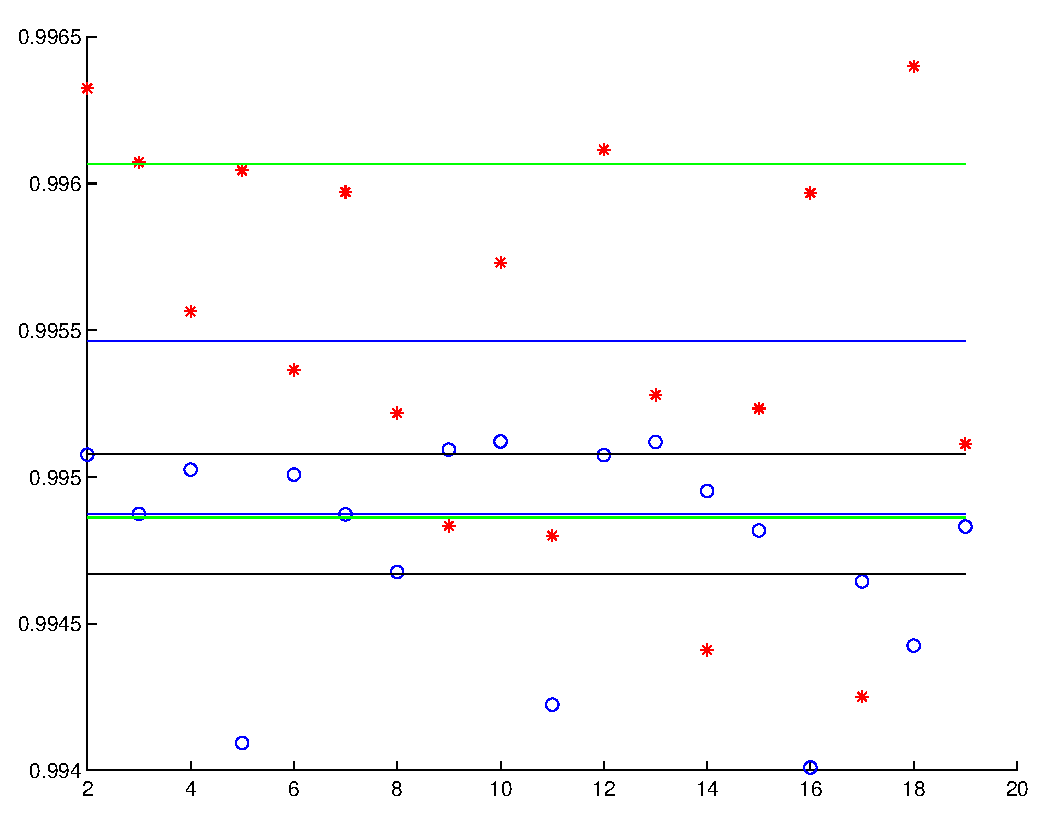
\includegraphics[width=1.00\linewidth]{Figures/fdllrep}
  \caption{The $18$ different settings for \bzip\ of the same setup}
  \label{fig:fdllrep}
\end{figure}

The blue lines in the figure show each median value for the geometric means, the green lines represent one standard deviation from the median for the \FDI\ case, while the black lines represent the standard deviation from the median for the \llvm\ case. As it can be seen, not only the values are too similar, varying only from the fourth decimal digit, but also the medians and their standard deviations overlap, collapse. This is a strong indicator that there is no significant difference between those measures.

So, to accomplish the task, just consider that a single-run experiment could have measured any one of the $3$-consecutive run values individually, moreover, a single run may have also collected the best, or the worst values for the actual times of the experiment. Hence, to outcome a speedup for \FDI\, collected the worst running time for \llvm\ inlined program, and the best running time for the \FDI\ inlined program.

Even though this biased data showed a speedup, it was really worthless, only $0.46 \%$. Therefore, to reinforce that the input set is also a big issue, the data were "adjusted", leaving the slowdowns and some of the tiny speedups gathered from the list of inputs off the final list to be shown. This way a tiny, but possibly measurable speedup, was presented in \refSection{sec:speedup}. Nevertheless, define a list of inputs is an issue and has to be treated as part of the experiment design, as this ``speedup'' have shown. That is why a complete list of inputs containing all the explanations is a requirement when presenting data as well. The full data for the "speedup" experiment are shown in table \refTable{tab:fullexp}.

\begin{table}
  \centering
  \begin{tiny}
  
\begin{tabular}{lllll}

{\bf Input} & {\bf Normalized \FDO} & {\bf Normalized \llvm} & {\bf Speedup} \\ \hline

auriel & 0.9720 & 1.0076 & 0.9647   \\ 
avernum & 0.9922 & 0.9905 & 1.0017 \\
cards & 0.9909 & 0.9989 & 0.9919  \\
ebooks & 0.9909 & 0.9920 & 0.9988  \\
gcc & 0.9966 & 1.0059 & 0.9907  \\ 
lib-a & 0.9940 & 0.9970 & 0.9970  \\ 
mohicans & 1.0000 & 1.0048 & 0.9951  \\
ocal & 0.9988 &1.0075 & 0.9913  \\ 
paintings & 1.0000 & 1.0051 & 0.9949  \\
potemkin & 0.9916 & 0.9887 & 1.0029  \\
proteins-1 & 0.9977 & 0.9910 & 1.0068  \\
proteins-2 & 0.9813 & 0.9950 & 0.9862  \\
revelation & 0.9868 & 0.9887 & 0.9980  \\ 
sherlock & 1.0000 & 1.0020 &1.0125  \\ 
usrlib & 1.0000 & 0.9875& 1.0458  \\  \hline
Speedup & & & 0.9953 (0.46 \%) \\

\hline
\end{tabular}

  \end{tiny}
  \caption{Summary of the normalized data used to produce a speedup for \bzip}
  \label{tab:fullexp}
\end{table}

On the other hand, in \refSection{sec:slowdown} the opposite was performed, choosing the worst individual running time for the \FDI\ inlined program and the best running time for the \llvm\ inlined program. Proceeding this way it was easy to present, from "a different" individual measuring, a slowdown. And as both results followed the same methodology, they are both correct, and this is unexplainable unless considering that there is variance on the data collected.

The same process was employed for the \gzip\ case, using $20$ different settings, the \refFigure{fig:gzipfdll} shows the data collected in a similar way of what was presented in \refFigure{fig:fdllrep}. In \refFigure{fig:gzipfdll} we can notice that there is possibly a slowdown compared to \llvm\ for this setup, and even though it was not hard to report a speedup.

\begin{figure}
  \centering
  \includegraphics[width=1.00\linewidth]{Figures/gzipfdll}
  \caption{The $20$ different settings for \gzip\ of the same setup}
  \label{fig:gzipfdll}
\end{figure}

These cases were artificially constructed using our empirical actual data, considering that if we used a single-run methodology these results could appear. But using \CP\ methodology, the researcher is able to correctly identify that there is no statistical difference between both inliners, for the setup proposed. This result, in a certain way, reinforces the result of ~\cite{Curtsinger2013}, where they reported no speedup of $-O2$ over $-O3$ for all benchmarks they analyzed, when code randomization is applied.

%=============== GCC

\subsubsection{Analysis of \gcc}

The same process was used for the \gcc\ case, the best running times for \FDI\ inlined program in the setting were selected, and the worst running times for \llvm\ inlined programs were also selected. These data were select for each input, and from this our speedup experiment was constructed. In a single-run framework it is perfectly reasonable that this result can actually appear. But in this case we came up with a result considering a somewhat reduced input set, which produced an even better speedup. Again, this was done to raise the question about the proper set of inputs to be employed. In fact, the set presented in \refSection{sec:speedup} was already an extract from the SPEC CPU 2006 benchmark suite.

In reality the full SPEC CPU 2006 benchmark suite was applied, and 4 more inputs, which were converted from the SPEC 2000 benchmark, were added fulfilling the 15-input set to each program, as described in \refSection{sec:description}. If the full input-set is taken, the experiment would have produced a different result, the speedup in the case of the best run-times, would be of $2.52 \%$, as shown in \refTable{tab:fullspeedup} and in \refFigure{fig:gccall}.

\begin{table}
  \centering
  \begin{tiny}
  
\begin{tabular}{lllll}

{\bf Input} & {\bf \FDO\ normalized} & {\bf \llvm\ normalized} & {\bf Speedup} \\ \hline

166 & 0.9532 & 0.9755 & 0.9771  \\
200 & 0.9594 & 0.9594 & 1.0000  \\
c-typeck & 0.9400 & 0.9845 & 0.9548  \\
cccp & 0.9646 & 0.9646 & 1.0000  \\
Cp-decl & 0.9589 & 0.9784 & 0.9800  \\
expr & 0.9208 & 0.9567 & 0.9624  \\
expr2 & 0.9208 & 0.9686 & 0.9506  \\
g23 & 0.9860 & 1.0441 & 0.9443  \\
integrate & 0.9810 & 1.0000 & 0.9810  \\
s04 & 0.9987 & 1.0153 & 0.9836  \\
scilab & 0.9886 & 0.9886 & 1.0000  \\
bzipR-all & 0.9907 & 1.0055 & 0.9852  \\
lbm-all & 0.9696 & 1.0303 & 0.9411  \\
mcf-all & 1.0000 & 1.0270 & 0.9736  \\
parser-all & 0.9970 & 1.0059 & 0.9911  \\  \hline
Geomean & & & 0.9748 (2.52 \%)\\
  
\hline
\end{tabular}

  \end{tiny}
  \caption{Summary of the normalized data used to produce a speedup for \gcc}
  \label{tab:fullspeedup}
\end{table}

\begin{figure}
  \centering
  \includegraphics[width=1.00\linewidth]{Figures/speedupgccall}
  \caption{The $20$ different settings for \gcc\ of the same setup}
  \label{fig:gccall}
\end{figure}

Therefore, the input-set matters, as much as a sound methodology. To summarize this section and illustrate the outcomes of our framework, employing \CP\ methodology \refFigure{fig:gcc-results} presents one of the figures automatically generated by the framework. In this figure it can be observed that there was no speedups, nor slowdowns for the \gcc\ case, the error bars present in \refFigure{fig:gcc-results} demonstrates the level of confidence in the geometric mean results.

As already mentioned, this figure was automatically generated by our system, and reflects the geometric mean of all inputs for twelve different \FDI\ inliners, the \llvm\ inliner (called static in the figure) and another static inliner called benefit.

\begin{figure}
  \centering
  \includegraphics[width=1.00\linewidth]{Figures/gcc-results}
  \caption{The actual result for \gcc\ returned by our \CP\ framework}
  \label{fig:gcc-results}
\end{figure}

%============ regular text

Next section (\refSection{sec:cmbprof}) describes the \CP\ methodology in more detail, explaining its use and how to measure the results, in order to avoid the problems highlighted by the example in \refSection{sec:speedup}.

	
\section{Reporting a speedup measured using \FDI\ }
	\label{sec:speedup}
	
We have performed an experiment comparing the performance of the \llvm\ static inliner and the \FDI\ inliner described in ~\cite{BerubePhD}. Both inliners are also evaluated with respect to the baseline Never, which means never inline. Our setting that was tested using the programs \bzip\ and \gzip, was not extracted from the SPEC CPU 2006 benchmark suite, rather than we used the fully-functional ``real'' versions. Using the real versions of the compressor programs eliminates the unrealistically-simplified profiling situation where mutually-exclusive use cases are combined into a single program run. Consequently, these programs cannot do decompression and compression, or multiple levels of compression, within the same run.  These distinct use-cases must be covered by different inputs in the program workload. Our results show a slight improvement over the \llvm\ results. For \gcc\ we used the SPEC CPU 2006 benchmark suite.  SPEC provides 11 inputs for \gcc\ from those we selected 7, {\tt 166, Cp-decl, expr, expr2, g23, integrate, bzipR-all, lbm-all, mcf-all}. And we added 3 inputs converted from the SPEC 2000 benchmark, \bzip, \lbm, and \mcf.

The \bzip\ and \gzip\ programs were executed using a representative set of inputs, where compression tasks and decompression tasks were tested under similar inputs.
The compression set contains the following inputs, with the compression level shown in parentheses:
\begin{itemize}

%\item {\tt avernum (-3)}: The installer for the demo version of the game  ``Avernum: Escape from the Pit'' from Spiderweb Software.

\item {\tt cards (-4)}: A collection of greeting card layouts in the TIFF (uncompressed) image format.

%\item {\tt ebooks (-5)}: A collection of ebooks, with and without images, and in a variety of formats, from Project Gutenberg\footnote{http://www.gutenberg.org}.

%\item {\tt potemkin-mp4 (-6)}: The 1925 movie ``Bronenosets Potyomkin (Battleship Potemkin)'' in MP4 format, from the Internet Archive\footnote{http://archive.org/details/BattleshipPotemkin}.

%\item {\tt proteins-1 (-7)}: A sample of 33 proteins from the RCSB Protein Data Bank database.  6 files for each protein, each stored in a different text-based format, provide different characteristics of the protein's structure\footnote{http://www.rcsb.org}.

\item {\tt revelation-ogg (-8)}: The audio book ``The Revelation of Saint John'' in OGG format, from Project Gutenberg\footnote{http://www.gutenberg.org/ebooks/22945}.

%\item {\tt usrlib-so (-9)}: A collection of shared object (.so) files from {\tt /usr/lib/} of a 32-bit gentoo-linux machine.

\end{itemize}

The decompression set for each compressor uses the same base set of files, pre-compressed by the appropriate compressor at the default compression level.  The decompression set is composed of:
\begin{itemize}
\item {\tt auriel}: The ``Auriel's Retreat'' land-mass addition mod by lance4791 for the game ``The Elder Scrolls IV: Oblivion'' from Bethesda Softworks\footnote{http://planetelderscrolls.gamespy.com/View.php?view=\\ \hspace*{150 pt}OblivionMods.Detail\&id=5949}.

%\item {\tt gcc-453}: The source-code archive of the \gcc\ compiler, version 4.5.3\footnote{http://gcc.gnu.org/gcc-4.5}.

%\item {\tt lib-a}: A collection of library files (.a) from {\tt /lib/} of a gentoo-linux machine.  As per the gentoo development guide, a library will be installed in {\tt /lib} (boot critical) or {\tt /usr/lib} (general applications), but not both\footnote{http://devmanual.gentoo.org/general-concepts/filesystem/index.html}.

%\item {\tt mohicans-ogv}: The 1920 movie ``Last of the Mohicans'' in OGV (ogg video) format, from the Internet Archive\footnote{http://archive.org/details/last\_of\_the\_mohicans\_1920}.

\item {\tt ocal-019}: The Open Clip Art Library archive, version 0.19. The images are primarily in vector-graphics formats\footnote{http://openclipart.org/collections}.

%\item {\tt paintings-jpg}: A collection of watercolor paintings, in JPG format.

\item {\tt proteins-2}: A completely different sample of 157 proteins from the RCSB Protein Data Bank database, each in 6 different file formats.

%\item {\tt sherlock-mp3}: The audio book ``The Adventures of Sherlock Holmes'' in MP3 format, from Project Gutenberg\footnote{http://www.gutenberg.org/ebooks/28733}.

\end{itemize}

\subsection{Setting up the experiments}

%============ Hardware

We ran our experiments on $20$ Dell Optiplex 755, whose characteristics are:
\begin{itemize}

\item Intel Duo Core E6750 2.66 GHz processor;

\item 4 GB RAM;

\item DVD-RW drive;

\item Intel Pro/1000 Gb ethernet;

\item Gigabyte GeForce 8600 video cards;

\item 250 GB SATA II drive. 

\end{itemize}

%============ Our results

\subsection{Presenting the results}

We employed a single-run methodology for the experiments and we used three benchmarks to test our hypotheses, \bzip, \gzip, and \gcc. The results are presented in the following way, we grouped the \bzip\ with \gzip, and separate \gcc\ to another section. We decided to present the results for \bzip\ and \gzip\ together because these programs have similar behavior and \gcc\ has a completely different behaviour.

\subsubsection{Compressors / Decompressors}

We will start by describing our experiments with the data collected from the \bzip\ runs are summarized in \refTable{tab:speedupb}. In this table we show that we achieved a slight speedup of $1.36 \%$ over \llvm\ results.

\begin{table}
  \centering
  \begin{tiny}
  
\begin{tabular}{lllll}

{\bf Input} & {\bf \FDO\ time (sec)} & {\bf Never time (sec)} & {\bf \llvm\ time (sec)} & {\bf Speedup} \\ \hline

auriel & 7.66 & 7.88 & 7.94 & 0.9647   \\ 
cards & 29.52 & 29.79 & 29.76 & 0.9919  \\
ocal & 44.94 & 44.99 & 45.33 & 0.9913  \\ 
proteins-2 & 79.6 & 81.11 & 80.71 & 0.9862  \\
revelation & 5.24 & 5.31 & 5.25 & 0.9980  \\  \hline
Geomean & & & & 0.9864 \\
  
\hline
\end{tabular}

  \end{tiny}
  \caption{Summary of the data collected during the experiment with \bzip}
  \label{tab:speedupb}
\end{table}

\refFigure{fig:speedup} shows the running time normalized by the time of Never (no inlining). We can see that the \FDI\ inliner outperforms Never and \llvm\ through all the inputs, which explains our speedup. The experiment on the program \bzip\ shed some light and these results can be fully explored in future research.

\begin{figure}
  \centering
  \includegraphics[width=1.00\linewidth]{Figures/speedupb}
  \caption{Running times of the \bzip\ inlined versions, normalized by Never}
  \label{fig:speedup}
\end{figure}

The final speedup, despite being a slight improvement, represents that the \FDI\ inliner can actually be employed instead of the \llvm\ inliner. And this result is significant because the program \bzip\ is small, simple, and not particularly fitted to inlining, leading to a conjecture that \FDI\ inliner are better than static ones. Which opens a wide range of experiments with other programs to confirm this conjecture. We ran also with \gzip, which happens to be quite similar to \bzip, and confirmed a speedup of $2.09 \%$ over \llvm\ results. These results can be seen in \refTable{tab:speedupz}, where the times are already normalized by the baseline Never (no inlining). \refFigure{fig:speedupz} shows the normalized running time for \gzip, and it also outperforms Never and \llvm through all inputs.

\begin{table}
  \centering
  \begin{tiny}
  
\begin{tabular}{lllll}

{\bf Input} & {\bf \FDO\ normalized} & {\bf \llvm\ normalized} & {\bf Speedup} \\ \hline

auriel & 0.9924 & 0.9924 & 1.0000   \\ 
cards & 0.9801 & 1.0092 & 0.9712  \\
ocal & 0.9914 & 1.0122 & 0.9794  \\ 
proteins-2 & 0.9905 & 1.0094 & 0.9811  \\
revelation & 0.9708 & 1.0072 & 0.9637  \\  \hline
Geomean & & & 0.9790 \\
  
\hline
\end{tabular}

  \end{tiny}
  \caption{Summary of the data collected during the experiment with \gzip}
  \label{tab:speedupz}
\end{table}

\begin{figure}
  \centering
  \includegraphics[width=1.00\linewidth]{Figures/speedup}
  \caption{Running times of the \gzip\ inlined versions, normalized by Never}
  \label{fig:speedupz}
\end{figure}

The results of the experiment are also consistent with other similar findings in the literature, whereas employing single-run experiments does not generate any kind of disturbance in the analysis, and the speedup result are statistically sound. So we can confirm a speedup over the static inliner for the \bzip\ and \gzip\ cases.

\subsubsection{\Gcc\ Benchmark}

For the \gcc\ benchmark we were able to report a more significant result, we measured a $5.88 \%$ speedup over \llvm\ using the set of inputs described above. This result is summarized in \refTable{tab:speedupgcc} below. The results are normalized by the baseline Never.

\begin{table}
  \centering
  \begin{tiny}
  
\begin{tabular}{lllll}

{\bf Input} & {\bf \FDO\ normalized} & {\bf \llvm\ normalized} & {\bf Speedup} \\ \hline

166 & 0.9532 & 0.9755 & 0.9771  \\
c-typeck & 0.9400 & 0.9845 & 0.9548  \\
Cp-decl & 0.9589 & 0.9784 & 0.9800  \\
expr & 0.9208 & 0.9567 & 0.9624  \\
expr2 & 0.9208 & 0.9686 & 0.9506  \\
g23 & 0.9860 & 1.0441 & 0.9443  \\
integrate & 0.9810 & 1.0000 & 0.9810  \\
s04 & 0.9987 & 1.0153 & 0.9836  \\
lbm-all & 0.9696 & 1.0303 & 0.9411  \\
mcf-all & 1.0000 & 1.0270 & 0.9736  \\  \hline
Geomean & & & 0.9630 \\
  
\hline
\end{tabular}

  \end{tiny}
  \caption{Summary of the data collected during the experiment with \gcc}
  \label{tab:speedupgcc}
\end{table}

The \refFigure{fig:speedupgcc} shows that the \FDI\ inliner outperforms Never and \llvm\ through all the inputs, the same way the former experiments did. But this particular experiment shows a much better result, for the speedup is much higher.

\begin{figure}
  \centering
  \includegraphics[width=1.00\linewidth]{Figures/speedupgcc}
  \caption{Running times of the \gcc\ inlined versions, normalized by Never}
  \label{fig:speedupgcc}
\end{figure}

Nevertheless, we can show how we can improve this result by just choosing less inputs from the original input set. In this case we can report a speedup of $7.76 \%$, as shown in \refTable{tab:speedupgcc1} and \refFigure{fig:speedupgcc1} below.

\begin{table}
  \centering
  \begin{tiny}
  
\begin{tabular}{lllll}

{\bf Input} & {\bf \FDO\ normalized} & {\bf \llvm\ normalized} & {\bf Speedup} \\ \hline

c-typeck & 0.9097 & 0.9745 & 0.9335  \\
expr & 0.9035 & 0.9552 & 0.9458  \\
expr2 & 0.8630 & 0.9660 & 0.8934  \\
g23 & 0.9119 & 0.9849 & 0.9259  \\
lbm-all & 0.8888 & 1.0000 & 0.8888  \\
mcf-all & 0.9487 & 1.0000 & 0.9487  \\  \hline
Geomean & & & 0.9224 \\
  
\hline
\end{tabular}

  \end{tiny}
  \caption{Extract of the data collected during the experiment with \gcc}
  \label{tab:speedupgcc1}
\end{table}

\begin{figure}
  \centering
  \includegraphics[width=1.00\linewidth]{Figures/speedupgcc1}
  \caption{Extract of the running times of the \gcc\ inlined versions, normalized by Never}
  \label{fig:speedupgcc1}
\end{figure}

\subsubsection{A slowdown}
\label{sec:slowdown}

We have to report also that the same experiment was carried out by another group, but unfortunately this group could not confirm our results. The differences in the timing measurements could be considered relevant, and both groups are now trying to understand what went wrong with the latter experiment. They measured a slowdown of $2.14 \%$ for \bzip, and a slowdown of $5.87 \%$ for \gzip, and a slowdown of $2.06 \%$ for \gcc,as shown in \refTable{tab:slowdownb}, \refTable{tab:slowdownz}, and \refTable{tab:slowdowngcc}.

\begin{table}
  \centering
  \begin{tiny}
  
\begin{tabular}{lllll}

{\bf Input} & {\bf Normalized \FDO} & {\bf Normalized \llvm} & {\bf Slowdown} \\ \hline

auriel & 0.9961 & 1.0025 & -0.64\%  \\
avernum & 0.9922 & 0.9905 & 0.18\%  \\
cards & 1.0457 & 0.9882 & 5.50\%  \\
ebooks & 0.9909 & 0.9920 & -0.11\%  \\
gcc & 0.9966 & 1.0059 & -0.93\%  \\
lib-a & 0.9940 & 0.9970 & -0.30\%  \\
mohicans & 1.0000 & 1.0048 & -0.48\%  \\
ocal & 1.0035 & 0.9984 & 0.51\%  \\
paintings & 1.0000 & 1.0051 & -0.51\%  \\
potemkin & 0.9916 & 0.9887 & 0.29\%  \\
proteins-1 & 0.9977 & 0.9910 & 0.68\%  \\
proteins-2 & 1.0012 & 0.9931 & 0.80\%  \\
revelation & 1.0359 & 0.9905 & 4.39\%  \\
sherlock & 1.0000 & 1.0020 & -0.21\%  \\
usrlib & 1.0000 & 0.9875 & 1.24\%  \\  \hline
Geomean & & & 0.71\% \\

\hline
\end{tabular}

  \end{tiny}
  \caption{Data reflecting a slowdown on \bzip\ -- collected by other research group}
  \label{tab:slowdownb}
\end{table}

\begin{table}
  \centering
  \begin{tiny}
  
\begin{tabular}{lllllll}

{\bf Input} & {\bf Normalized \FDO} & {\bf Normalized \llvm} & {\bf Slowdown} \\ \hline

avernum & 1.0093 & 1.0062 & 0.31\%  \\
cards & 1.0092 & 1.0092 & 0.00\%  \\
ebooks & 1.0081 & 1.0081 & 0.00\%  \\
potemkin-mp4 & 1.0052 & 1.0079 & -0.26\%  \\
proteins-1 & 1.0203 & 1.0064 & 1.37\%  \\
revelation-ogg & 1.0072 & 1.0072 & 0.00\%  \\
usrlib-so & 1.0651 & 1.0016 & 5.96\%  \\
auriel & 1.1363 & 0.9924 & 2.67\%  \\
gcc-453 & 1.1111 & 1.0085 & 9.23\%  \\
lib-a & 1.0735 & 1.0151 & 5.44\%  \\
mohicans-ogv & 1.2835 & 0.9269 & 27.78\%  \\
ocal-019 & 1.1412 & 1.0122 & 11.31\%  \\
paintings-jpg & 1.1826 & 0.9561 & 19.15\%  \\
proteins-2 & 1.0780 & 1.0074 & 6.55\%  \\
sherlock-mp3 & 1.2692 & 0.9411 & 25.85\%  \\  \hline
Geomean & & & 8.84\% \\

\hline
\end{tabular}

  \end{tiny}
  \caption{Data reflecting a slowdown on \gzip\ -- collected by other research group}
  \label{tab:slowdownz}
\end{table}

\begin{table}
  \centering
  \begin{tiny}
  
\begin{tabular}{lllllll}

{\bf Input} & {\bf \FDO\ normalized} & {\bf \llvm\ normalized} & {\bf Speedup} \\ \hline

166 & 0.9755 & 0.9755 & 1.0000  \\
c-typeck & 0.9845 & 0.9845 & 1.0000  \\
Cp-decl & 0.9784 & 0.9784 & 1.0000  \\
expr & 0.9686 & 0.9567 & 1.0124  \\
expr2 & 0.9686 & 0.9686 & 1.0000  \\
g23 & 1.0574 & 1.0441 & 1.0127  \\
integrate & 1.0253 & 1.0000 & 1.0253  \\
bzipR-all & 1.0315 & 1.0055 & 1.0258  \\
lbm-all & 1.0909 & 1.0303 & 1.0588  \\
mcf-all & 1.1081 & 1.0270 & 1.0789  \\   \hline
Geomean & & & 1.0210 \\

\hline
\end{tabular}

  \end{tiny}
  \caption{Data reflecting a slowdown on \gcc\ -- collected by other research group}
  \label{tab:slowdowngcc}
\end{table}


\section{Related Work}
	\label{sec:related}
	
There are several researchers concerned with the problem of reliability in performance measures. Kalibera \etal\ \cite{Kalibera2013} propose a rigorous methodology for measuring time, and claim that the measurements are still done in reasonable time. Their methodology considers that the environment, consisting of hardware and software, versions of the operating system, versions of the compiler used to measure data, they all change scarcely. For this reason their methodology asserts that before starting to take any measurement the whole environment has to be deeply investigated to find how many repeated iterations are required to achieve an independent state (the execution times of benchmark iterations are statistically independent). They provide means to calculate the number of runs are needed to achieve independent states for a benchmark analysis, also for measuring speedups. They used different benchmarks in their experiments and showed that there are different number of repetition counts for them. Our methodology does not assume that the environment changes scarcely, and we don't need a huge number of repetitions.

Mytkowicz \etal\ \cite{Mytkowicz2009} ran some experiments using SPEC CPU benchmarks and found significant systematic measurement errors in some sources, that could produce biased results. Their suggestion is to randomise the experimental setup to eliminate the bias. The idea of ramdomising is fully incorporated in Stabiliser \cite{Curtsinger2013}. Stabiliser is an LLVM-based compiler and runtime environment for randomisation of code, stack and heap layout. The purpose of randomisation is to reduce the need for repeated execution. Randomising the whole program in fact introduces more variation than in real systems, also some compiler transformations can become useless. Our approach is much less intrusive than theirs and we don't break compiler transformations.

Georges \etal\ \cite{Georges2007} shows that different methodologies can lead to different conclusions. They work with Java benchmarks and recommends running multiple iterations of each Java benchmark within a single VM execution, and also multiple VM executions. Our work is not focused in Java, but their recommendation remains true, it is necessary to use a reliable experimental methodology.

%============== Old text

\subsection{\FDO-related}

Most compilers take a single-run approach to \FDO: a single training run
generates a profile, which is used to guide compiler transformations.
Some profile file formats support the storage of multiple profiles
(\eg, \llvm), but when such a file is provided to a compiler, either
all profiles except the first are ignored, or a simple sum or average
is taken across the frequencies in the collected profiles.

Input characterization and workload reduction are not new problems.
However, the similarity metrics used for clustering
in \cite{BerubePhD} are unique in their applicability to
workload reduction for an \FDO\ compiler.  Most input similarity and
clustering work is done in the area of computer architecture, where
research is largely simulation-based, thus necessitating small
workloads of representative programs using minimally-sized inputs. The
architectural metrics of benchmark programs are repeatedly scrutinized
for redundancy, while smaller inputs are compared with large
inputs. Alternatively, some work bypasses program behavior and
examines the inputs directly.

Arnold \etal. present an inlining strategy similar to that used in
modern compilers~\cite{Arnold00}. They use a call-site sensitive call
graph profile, thus allocating procedure executions frequencies to
individual call sites.  Using code size expansion as the cost and
call site frequency as the benefit, call sites are inlined in
decreasing cost/benefit order up to a code expansion limit.  They
find that a 1\% code size expansion limit accounts for 73\% of dynamic
calls and reduces execution time by 9\% to 57\%.

Arnold \etal. use histograms to combine the profile information
collected by a Java JIT system over multiple program
runs~\cite{ArnoldOOPSLA05}.  The online profiler detects hot methods
by periodically sampling the currently-executing method.  After each
run of a program, histograms for the hot methods stored in a profile
repository are updated.

Salverda \etal\ model the critical paths of a program by generating
synthetic program traces from a histogram of profiled branch
outcomes~\cite{SalverdaCGO08}. To better cover the program's
footprint, they do an ad-hoc combination of profiles from SPEC
training and reference inputs.  In contrast, combined profiling and
hierarchical normalization provide a systematic method to combine
profile information for multiple runs.

Savari and Young build a branch and decision model for branch
data~\cite{SavariYoungJIPL00}.  Their model assumes that the next
branch and its outcome are independent of previous branches, an
assumption that is violated by computer programs (\eg, correlated
branches).  One distribution is used to represent {\em all events}
from a run; distributions from multiple runs are combined using
relative entropy --- a sophisticated way to find the weights for a
weighted geometric average across runs.
The model cannot provide
specific information about a particular branch, which is exactly the
information needed by \FDO.  However, this information is provided by
combined profiles because each event is represented separately.


\section{Conclusion}
	\label{sec:conclusion}
	
As mentioned in \refSection{sec:intro} a case study was proposed to study the inlining transformation. The experiment was designed to make a clear point about applying single-run methodologies and also about the definition of the input-set. Our experiment compared the \CP\ process with the single-run process. Any other transformation could have been chosen, because the \CP\ methodology can be applied in all general cases.

In \refSection{sec:speedup} it was shown an erroneous speedup, considering that it was measured by a single-run experiment. It was constructed considering that any of the measurements that ran independently could have happened in a single-run experiment. Hence searching the collected data it was not hard to find some outliers, or at least some data at extreme points. So, gathering these data points and defining two specific cases: \name{Best-runtime} and \name{Worst-runtime} for our \FDO-based inliner, and for a static inliner, in this case the \llvm\ inliner.

With these data points just selecting the ideal pairs it is possible to create the illusion of a speedup and a slowdown:
\begin{itemize}
 \item \name{Best-runtime} for \FDO\ and \name{Worst-runtime} for \llvm, creating a speedup;
 \item \name{Worst-runtime} for \FDO\ and \name{Best-runtime} for \llvm, creating a slowdown.
\end{itemize}

With these pairs and assuming a single-run methodology, it was not hard to produce a statistical analysis showing a speedup (or slowdown), and, it is worth to state again, for this experiment these pairs of data can be devised as being representative cases of single-run experiments. Therefore, each pair (speedup or slowdown) can be viewed as a result of a single-run experiment. Even if the researcher is extremely cautious the methodology is error-prone, a bias can be introduced without the knowledge, or intention, of the researcher. So the real message is to define and use a reliable methodology based on solid statistical measurements.

With our experiments some of the open questions posed in the \refSection{sec:intro} can be answered. We know for sure, and showed it in \refSection{sec:robust}, that \FDI\ decisions can be more accurate using \CP\ instead of single-run evaluation. For the case of the impact of \CP\ in a controlled case study, we can definitely state that as each program was run more than once, that's the price to pay for more reliability, but the impact is acceptable if the number of repetitions is not too high. In our experiments running three times was enough.

\subsection{Future work}

For future work our plans can be divided in two different paths:
\begin{itemize}
\item {\it Fine-tuning} Using the \CP\ methodology fine tune our \FDI\ inliner for some different benchmarks. We have already finished some experiments and now we are defining some changes in our algorithms;

\item {\it Apply \CP}  Applying \CP\ to different compiler transformations is another research path.

\end{itemize}


%\section*{Acknowledgments}
%	\input{text/ack}

%\bibliographystyle{latex8}
%%\bibliographystyle{abbrv}
\bibliographystyle{IEEEtran}
\bibliography{local}


\end{document}
